\documentclass{article}

\usepackage[margin=1in]{geometry}
\usepackage{amsmath,amssymb}
\usepackage[table,xcdraw]{xcolor}
\usepackage{graphicx}
\usepackage{caption}
\usepackage{subcaption}
\usepackage{float}

\graphicspath{ {ReportImages/OneClassSVM/} }


\begin{document}

\title{Autonomous Agents\\
Assignment 2: \emph{Single Agent Learning}}
\author{
Artur Alkaim -- 10859368\\
Peter Dekker -- 10820973\\
Rafael Reia -- 10859454\\
Yikang Wang -- 10540288\\
}
\maketitle
\section{Introduction}
In this assignment, we study the application of \emph{reinforcement learning
algorithms}. The main focus of this study is on the Q-Learning algorithm. We discuss the use of an $\epsilon$-policy and other policies.

Our goal is to tune the algorithms with the different parameters and understand how these parameters affect the performance that in this specific instance is determined by the number of steps the predator needs to catch the prey and how we can improve that by learning. 

\section{Program design}
In this assignment the overall progam design stays the same as in assignment 1, as we just added the equivalent classes for the new algorithms. So we have a new main class, \emph{MainQl} that, like the others, creates a specific environment for the predator and prey to live. Then it runs the simulation for that setup.

We also added a utility class to create graphs to measure the performance of different parameter settings. The library used is \emph{JFreeChart}. The code of the graph generation class is an adaptation of an online example, suited to the needs of our project.

\section{Evaluation}

%- Why? 'In order to test\ldots'
%- How? ' we ran \ldots N times on X computer'
%- What does it show?
%- Take home message

In order to test how the Q-learning algorithm works with different parameters we
have run our implemetation and computed the average of $100$ runs, each of them
with $10000$ episodes. With the averaging we have been able to get smoother
graphs.

\subsection{Different learning rates ($\alpha$)}
In order to test the influence of $\alpha$ we ran our implementation with
different values. The values used are:
$0.1 , 0.2, 0.3, 0.4$ and $0.5$. 

We have noticed that, as expected, when we increase the value of $\alpha$, the 
algorithm converges faster to an optimal value. A higher $\alpha$  makes the agent
consider the known information. If we choose $0$ for $\alpha$ the agent
would not learn anything, as it would just use the old (inital) values.

In theory we could increase $\alpha$ to $1$ to maximize the learning rate. However, we cannot trust on only learning, because transitions are non-deterministic, since the agent does not control the prey.

Thus, we should set the values as high as possible while considering this tradeoff.
We experimented with values from $0.1, \ldots , 0.5$. The results are
better with $0.5$ as the chart shows. They all converge, but with higher values
they converge faster. The average value shows how fast they converge, because if
a line converges faster, the number of low values will be high and this has a
direct impact on the average.

\begin{figure}[htbp]
\centering
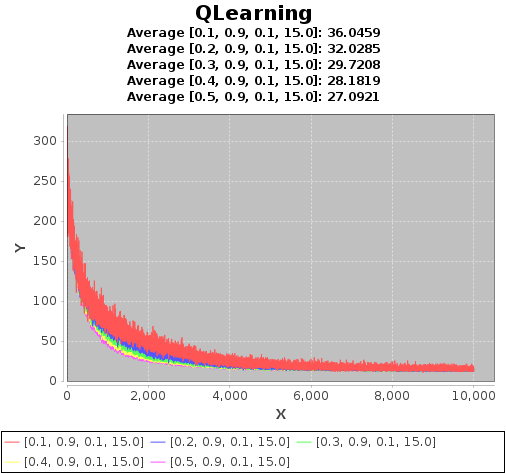
\includegraphics[width=0.8\textwidth]{res/alpha_01_to_05_gama_09_epsilon_01_IV_15.png}
\end{figure}

\subsection{Different discount factors ($\gamma$)}
We started to experiment with different values of $\gamma$. The values used are:
$0.2, 0.5, 0.7$ and $0.9$. 

The discount factor influences the importance that is given to future rewards.
This means that the lower the value, the less the agent cares about future
rewards and considers the immediate reward more. In the limit, if it is set to $0$ (zero), the agent only considers the immediate reward.

In this problem instance the immediate reward is almost always zero, so if we
have low $\gamma$ the learned values will be close to zero, i.e. it will not
learn anything. 

Thus, we noticed that by increasing $\gamma$ the number of steps converge to
lower values but do not have a big impact on the convegence rate.

\begin{figure}[htbp]
\centering
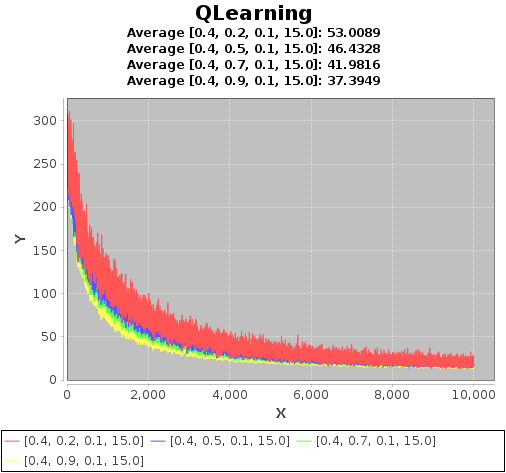
\includegraphics[width=0.8\textwidth]{res/alpha_04_gama_02_to_09_epsilon_01_IV_15.png}
\end{figure}

The chart shows what we just mentioned, that with higher values for $\gamma$, the line converges to a lower point.

\subsection{Different Initial Values}
We started to experiment with different values of IV. The values used are:
$0, 1, 15$ and $50$. 

As Q-learning is an iterative process, and we assign initial values to the
states, we have to consider what values we use and the impact it may have on the
performance/evolution of the process.

It has been shown that high values for the initialization, known as \emph{optimistic
initial conditions}, can encourage exploration. This is positive because after
the agent explores all the states and assigns the values for those states, it can
start optimizing paths.
With low initial values, consequently low exploration, the number of states that
still have the initial values are higher throughout the process. When the agent
is surrounded by states with the same value, it will choose randomly. This causes a
behaviour closer to a random policy at the begining. Therefore, the first group of
iterations for low initial values has a much higher number of steps than when using \emph{optimistic
initial conditions}.

\begin{figure}[htbp]
\centering
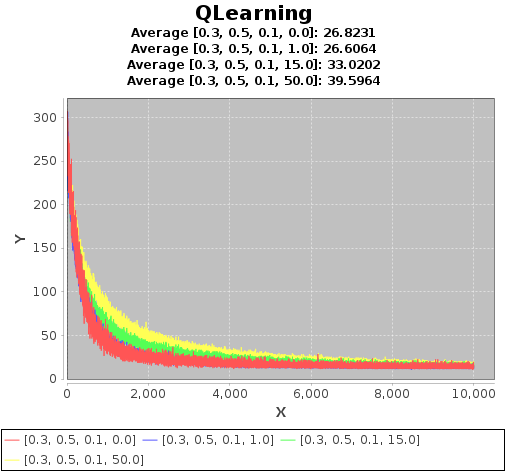
\includegraphics[width=0.8\textwidth]{res/alpha_03_gama_05_epsilon_01IV_00_to_50.png}
\end{figure}

\section{Policy}
The main policy used was the $\epsilon-greedy$ policy. We will discuss the effect of using different values for $\epsilon$ in section \ref{ep}.

The results using a different policy, the \emph{softmax} policy, are described in section \ref{softmax}.

\subsection{Different $\epsilon$'s}
\label{ep}
In order to understand the impact of $\epsilon$ to our implementation we run
in with the following values:
$0.1, 0.3, 0.5$ and $0.7$.

$\epsilon$ is a parameter of the $\epsilon-greedy$ policy and not directly of the Q-Learning algorithm. The tests in this section show mostly how the chosen policy can
influence the learning process and its outcomes. 

As this parameter is related to the probability of choosing a random action over
the maximum valued action, it determines whether more exploration or exploitation is pursued.

If $\epsilon$ is increased, the behaviour is closer to a random
policy, but contrary to what happens with the initial values, this policy has
impact throughout the process and not just at the beginning.

Higher $\epsilon$ values give worse convergence, as can be seen in the following
chart.

\begin{figure}[htbp]
\centering
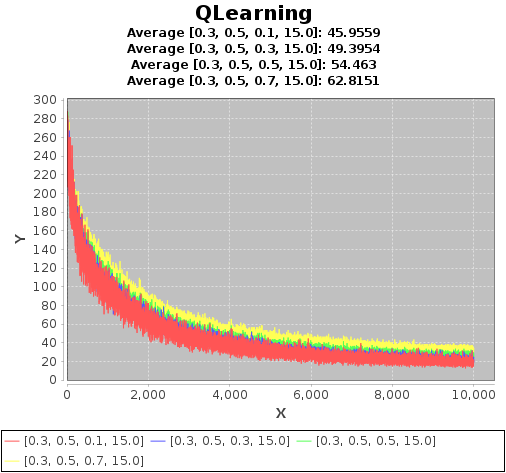
\includegraphics[width=0.8\textwidth]{res/alpha_03_gama_05_epsilon_01_to_07_IV_15.png}
\end{figure}

\subsection{Softmax}
\label{softmax}

This policy calculates the probablities for each action to be chosen at each
timestep. This algorithm can be tuned through the parameter $\tau$, which is
called \emph{temperature}.
The temperature is a positive value that has impact on the result of the
formula.

With high $\tau$ the probability of all actions is (nearly) equal, causing
this to have a nearly random behaviour.

As $\tau \rightarrow 0$ the behaviour is the same as the $\epsilon-greedy$
policy.
So this policy works with a tradeoff, trying to balance totally random choices with a purely greedy approach.

The results presented in the graph show that with higher $\tau$ the number of
steps is very high, as expected, caused by the nearly random behaviour. With low
values, $1 or 0.1$ the final number of steps is close to the best that we got
with the $\epsilon-greedy$ policy. This is expected as explained before.

\begin{figure}[htbp]
\centering
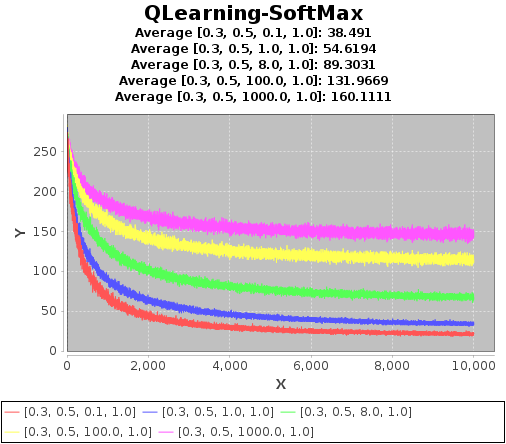
\includegraphics[width=0.8\textwidth]{res/alpha_03_gamma_05_temp_01_to_1000_IV_1.png}
\end{figure}

Again in order to test the impact of changing the parameters for the Q-Learning,
we ran again with the same configuration as before, with different values for
$\alpha, \gamma and \tau$. 
The impact of  $\alpha and \gamma$ are the same as previous with any value of
$\tau$.

\section{Conclusion}

In this assignment, the full pipline of Q-learning as well as Softmax version Q-learning is implemented. Based on these two algorithms, a series of experiment with different parameter settings were done. According to the results of the experiments, we found that finding the right combination of parameters is useful, because it can greatly speed up converge and also improve the performance.

\end{document}
